\section[Overall Description]{\hyperlink{toc}{Overall Description}}

\subsection[Product Perspective]{\hyperlink{toc}{Product Perspective}}
	Thanks to the general introduction and the scope definition of the system from the previous sections, we are now able to describe the interfaces that
	our system has to deal with and then the definition of the model's structure in order to interact with the given interfaces; at the end of the section \textbf{state diagrams} 
	are used to emphasize the dynamic behavior of the most critical classes.
	\subsubsection[System Interfaces]{\hyperlink{toc}{System Interfaces}}
		\label{sec:systemInterfaces}
		SafeStreets offers an interface to its users that can be users and authorities to provide them its basic and advanced functionalities. All the data needed to authenticate
		the users will be managed inside the system as well as the information of the parking violations that will be mined and crossed.\\
		
		To accomplish the \hyperref[sec:goals]{\textcolor{blue}{goals}} stated in the \hyperref[sec:introduction]{\textcolor{blue}{introduction}} the application needs also to interact with three main external interfaces as reported in the following picture (\autoref{fig:systemInterfaces}).  
		\vspace{0,3cm}
		
		\begin{figure}[h]
			\centering
			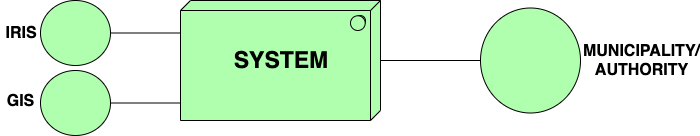
\includegraphics[scale=0.5]{/diagrams/systemInterfaces.png}
			\caption{\label{fig:systemInterfaces}System Interfaces}
		\end{figure}
		
		Two different kinds of interfaces are distinguished in the picture above:
		\begin{itemize}
			\item \textbf{Left hand side:} interfaces that provide APIs needed by the system to perform internal operations. 
			
			In particular:
			\begin{itemize}
				\item \textsc{IRIS} is used to process the image received in a violation to read the plate of the vehicle. Whenever a violation is received, in fact, if all other data is provided correctly the system needs to try reading the plate to check if it coincides with the one inserted by the user. Thanks to the image recognition the system is able to discard inconsistent information relative to the plate or retrieve it when missing. 
				\item \textsc{GIS} is used to retrieve the name of the street where the violation has been reported and to highlight the streets where the most parking violations occur or the unsafe areas of a municipality. In the system it is first important to find the exact position of an infraction in order to provide it to the authorities but also to store this information as it can be mined and crossed in the other functionalities. 
			\end{itemize}
			\item \textbf{Right hand side:} interfaces that enable the system to send and receive data to the authorities. 
			
			In particular when:
			\begin{itemize}
				\item The reported violation has been accepted by the system and enriched with the metadata that can be useful to the authority. In this case the correct information is sent to the authority interested in the area that contains the related position.
				\item The municipality provides information about the accidents that occur in its area. Received data is crossed by the system to determine the safety of its streets. Thanks to this additional operation the application is also able to determine the best interventions for unsafe areas and suggest them to its users.
			\end{itemize}
		\end{itemize}
	
	\subsubsection{Model Structure}
	The static analysis now continues to define the internal structure of the system, in particular with a high-level class diagram that shows the most important objects and their relations in order to achieve the \hyperref[sec:goals]{\textcolor{blue}{goals}}.\\
	
	The main objects in the UML diagram (\autoref{fig:classDiagram}) are:
	\begin{itemize}
		\item \textbf{Customer}
		\item \textbf{User}
		\item \textbf{Authority}
		\item \textbf{Registration} \todo{per me qua ci sta un bel pattern per fare la registrazione diversa per utente diverso}
		\item \textbf{Violation}
		\item \textbf{ParkingViolation}
		\item \textbf{Position}
		\item \textbf{Street}
		\item \textbf{Area}
	\end{itemize}
	
	\begin{figure}[h!]
		\centering
		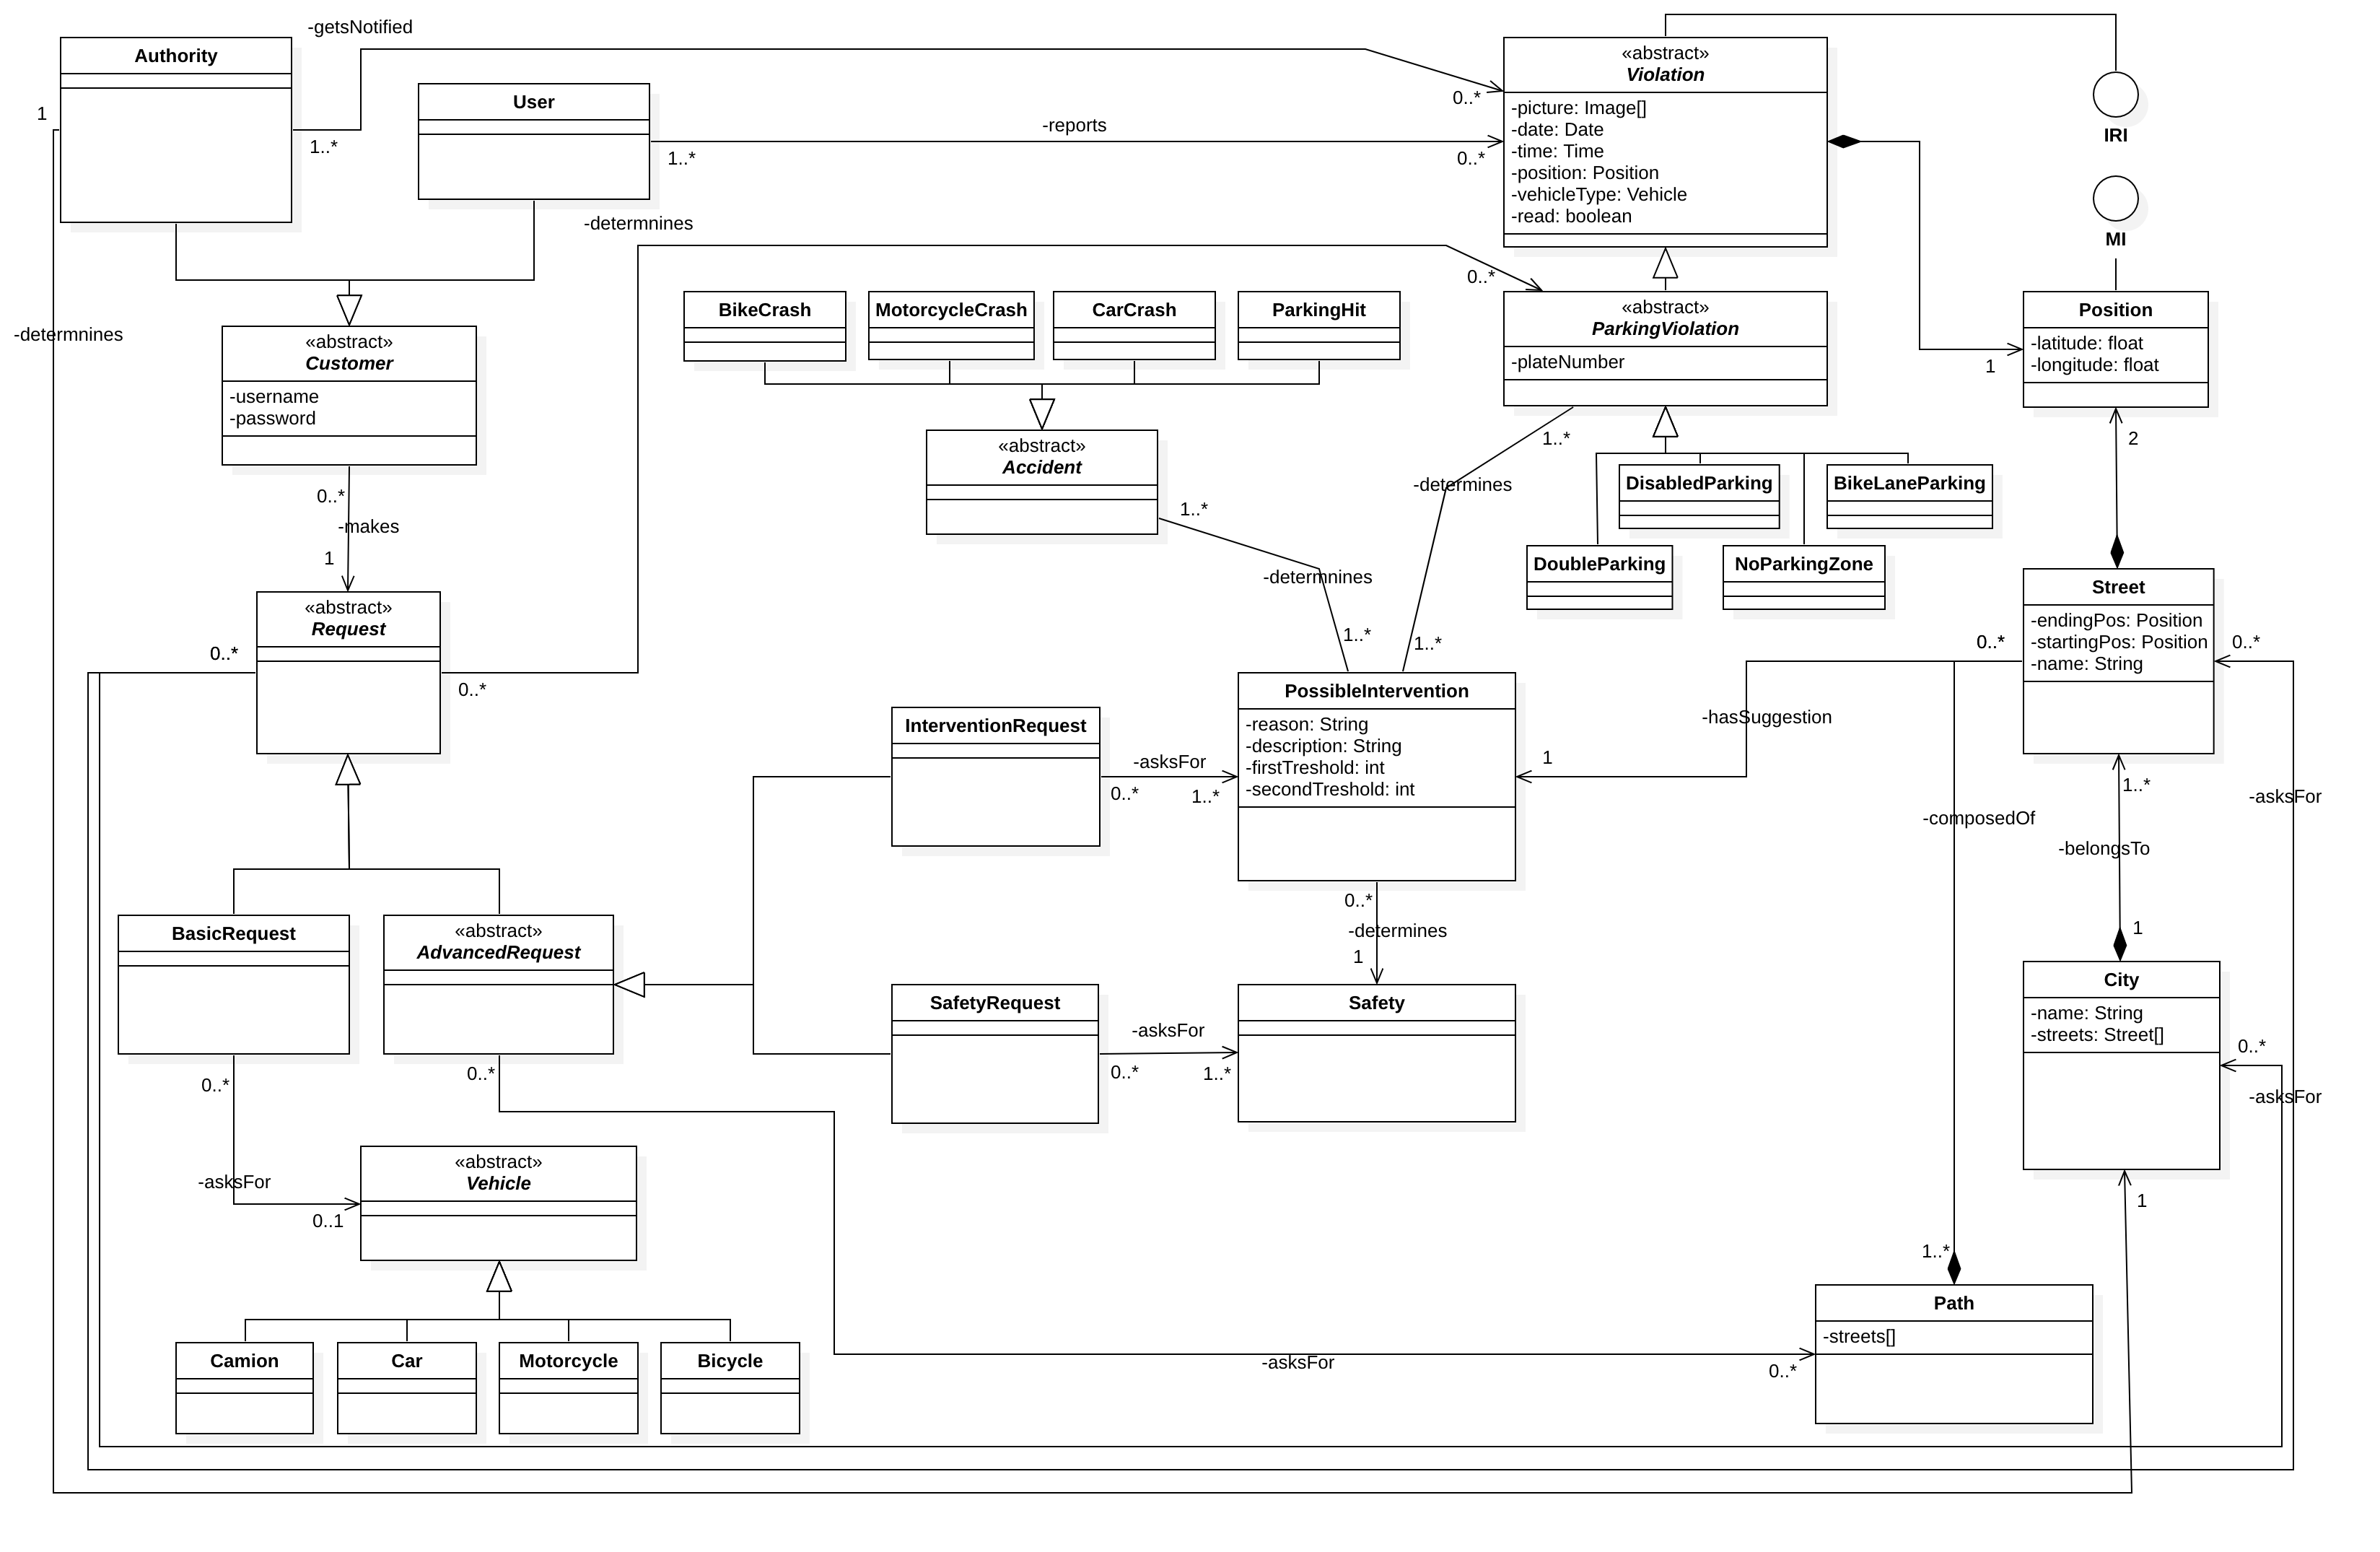
\includegraphics[width=\linewidth]{/diagrams/classDiagramModel.png}
		\caption{\label{fig:classDiagram}High-level model structure}
	\end{figure}

\subsection[Product Functions]{\hyperlink{toc}{Product Functions}}

\subsection[User Characteristics]{\hyperlink{toc}{User Characteristics}}

\subsection[Domain Assumptions]{\hyperlink{toc}{Domain Assumptions}}

\subsection[The World and the Machine]{\hyperlink{toc}{The World and the Machine}}